% !TEX program = xelatex
% EECS 245: Mathematics for Machine Learning, Winter 2026 Final Exam
\documentclass[11pt]{article}
\usepackage{../../eecs245}

% Uncomment the line below to show solutions in gray boxes
\enablesolutions

% Uncomment the line below to include student name/uniqname section
\enablestudentinfo

% Enable exam mode to include UMID and room options
\enableexam

\usepackage{amsmath, amsfonts, amssymb, multicol, hyperref}

% Restore Computer Modern for math
\DeclareSymbolFont{operators}{OT1}{cmr}{m}{n}
\DeclareSymbolFont{letters}{OML}{cmm}{m}{it}
\DeclareSymbolFont{symbols}{OMS}{cmsy}{m}{n}

\makeatletter
\renewcommand{\@probheader}[1]{%
  \ifx#1\@empty
    Problem~\theproblem%
  \else
    Problem~\theproblem\ #1%
  \fi
}
\makeatother

% Metadata
\newcommand{\coursename}{EECS 245}
\newcommand{\term}{Winter 2026 at the University of Michigan}
\newcommand{\assignment}{Final Exam}
\newcommand{\duedate}{}
\newcommand{\submissioninstructions}{

\textbf{Instructions}

\begin{itemize}
\item This exam consists of 13 problems, worth a total of 130 points, spread across 14 pages (7 sheets of paper). \textbf{All problems count towards your Final Exam score; certain problems also count towards your Midterm 1 or Midterm 2 redemption scores.}
\item You have 120 minutes to complete this exam, unless you have extended-time accommodations through SSD.
\item Write your uniqname in the top right corner of every page in the space provided.
\item For free response problems, you must show all of your work (unless otherwise specified), and $\boxed{\text{circle}}$ your final answer. We will not grade work that appears elsewhere, and you may lose points if your work is not shown.
\item For multiple choice problems, completely fill in bubbles and square boxes; if we cannot tell which option(s) you selected, you may lose points. \\
\bubble{A bubble means that you should only select one choice.} \\
\squarebubble{A square box means you should select all that apply.}
\item You may refer to \textbf{3} two-sided handwritten notes sheets. Other than that, you may not refer to any other resources or technology during the exam (no phones, watches, or calculators).
\end{itemize}

}

\begin{document}
\makemytitle{\coursename}{\term}{\assignment}{}
{\submissioninstructions}
{\bubble{1013 DOW} \bubble{1017 DOW} \bubble{2725 BBB} \bubble{Other}}

\vspace{1em}

You are to abide by the University of Michigan/Engineering Honor Code. To receive a grade,
please sign below to signify that you have kept the Honor Code pledge.

\textit{I have neither given nor received aid on this exam, nor have I concealed any violations of the Honor Code.}

\emptybox{1.5cm}

\newpage

\begin{center}
\:

\vspace{9cm}
This page has been intentionally left blank.
\end{center}

\newpage

% \textbf{Tip: Skim through the entire exam before starting to work on it.}

\begin{prob}[(12 pts) \hfill $\boxed{\text{Counts towards Midterm 1 redemption score}}$]
Suppose we'd like to find the optimal constant prediction, $w^*$,
for the constant model $h(x_i) = w$, given the following dataset of $n = 4$ values.
$$y_1 = 3, \quad y_2 = 6, \quad y_3 = 6, \quad y_4 = 13$$
In each part, choose from the options below.

\[
\begin{array}{l@{\hspace{1.75cm}}l}
A = 3 & E = 7 \\[1.5ex]
B = \dfrac{4}{\frac{1}{3} + \frac{1}{6} + \frac{1}{6} + \frac{1}{13}} \approx 5.37 & F = \sqrt{\dfrac{3^2 + 6^2 + 6^2 + 13^2}{4}} \approx 7.90 \\[3ex]
C = 6 & G = 8 \\[1.5ex]
D = \left( 3 \cdot 6 \cdot 6 \cdot 13 \right)^{1/4} \approx 6.12 & H = 13 \\
\end{array}
\]

\begin{enumerate}[label=(\roman*)]
\item (3 pts) What value of $w^*$ minimizes $R(w) = \displaystyle \frac{1}{4} \sum_{i=1}^4 (y_i - w)^2$? \\

\bubble{$A$} \bubble{$B$} \bubble{$C$} \bubble{$D$} \correctbubble{$E$} \bubble{$F$} \bubble{$G$} \bubble{$H$} \\

\begin{solution}
For (i), the minimizer of mean squared error is the mean, so
\[
w^* = \frac{3+6+6+13}{4} = \boxed{7}
\]
\end{solution}

% \item What value of $w^*$ minimizes $R(w) = \displaystyle \frac{1}{4} \sum_{i=1}^4 (y_i^2 - w^2)^2$? \\
% \bubble{$A$} \bubble{$B$} \bubble{$C$} \bubble{$D$} \bubble{$E$} \bubble{$F$} \bubble{$G$} \bubble{$H$} \\

\item (3 pts) What value of $w^*$ minimizes $R(w) = \displaystyle \lim_{p \to \infty} \displaystyle \frac{1}{4} \sum_{i=1}^4 |y_i - w|^p$? \\
\bubble{$A$} \bubble{$B$} \bubble{$C$} \bubble{$D$} \bubble{$E$} \bubble{$F$} \correctbubble{$G$} \bubble{$H$} \\

\begin{solution}
For (ii), as $p \to \infty$, the largest value of $|y_i-w|$ dominates. So we should put $w$ halfway between the smallest and largest data values, as discussed in \href{https://notes.eecs245.org/introduction-to-supervised-learning/comparing-loss-functions/\#beyond-absolute-and-squared-loss}{Chapter 1.4}.
\[
w^* = \frac{3+13}{2} = \boxed{8}
\]
\end{solution}

\item (3 pts) What value of $w^*$ minimizes $R(w) = \displaystyle \frac{1}{4} \sum_{i=1}^4 (\log(y_i) - \log(w))^2$? \\
\bubble{$A$} \bubble{$B$} \bubble{$C$} \correctbubble{$D$} \bubble{$E$} \bubble{$F$} \bubble{$G$} \bubble{$H$} \\

\begin{solution}
For (iii), let $u=\log(w)$. The problem is now asking for the best constant prediction for the transformed values $\log(y_i)$, so
\[
u^* = \frac{\log(3)+\log(6)+\log(6)+\log(13) = \log(3 \cdot 6 \cdot 6 \cdot 13)}{4}
\]
Exponentiating gives
\[
w^* = e^{u^*} = \boxed{(3 \cdot 6 \cdot 6 \cdot 13)^{1/4}}
\]
This was also a homework problem.
\end{solution}

\item (3 pts) The slope of the graph of $R(w) = \displaystyle\frac{1}{4} \sum_{i = 1}^4 |y_i - w|$ at $w = \alpha$ is $-1/2$. Among the options above, which could be $\alpha$? \\

\bubble{$A$} \correctbubble{$B$} \bubble{$C$} \bubble{$D$} \bubble{$E$} \bubble{$F$} \bubble{$G$} \bubble{$H$} \\
\begin{solution}
For (iv), the slope of mean absolute error at any $w$ that is not a data point is

$$\frac{\text{\# left of } w - \text{\# right of } w}{n}$$

Here, in order to achieve a slope of $-1/2$, we need to have 1 data point to the left of $w$ and 3 to the right, since $\frac{1-3}{4} = -1/2$. This means we need $w$ to be between $3$ and $6$, \textbf{exclusive}. The only value in this interval is $B$,

\[
\boxed{\dfrac{4}{\frac{1}{3}+\frac{1}{6}+\frac{1}{6}+\frac{1}{13}} \approx 5.37}
\]

\end{solution}
\end{enumerate}    

% \begin{subprob}(XX pts)
% Consider a dataset of $n$ values, $y_1, y_2, \ldots, y_n$, with mean $\bar y$.

% Define
% \[
% R(w) = \frac{1}{n} \sum_{i=1}^n \left(2(y_i - w)^2 + (y_i - (12 - w))^2\right)
% \]

% Show that the value of $w$ minimizing $R(w)$ depends only on $\bar y$, and find that value.

% \emptybox{6.5cm}{}

% \end{subprob}

% \begin{subprob}(XX pts)
% Consider a dataset of $n$ values, $y_1, y_2, \ldots, y_n$.

% What value of $w$ minimizes the following function?
% \[
% R(w) = \frac{1}{n} \sum_{i=1}^n \left(y_i^6 - (w - 1)^3\right)^2
% \]

% \textit{Hint: There is no need to use calculus here}

% \bubble{$1 + \left(\frac{1}{n} \sum_{i=1}^n y_i^6\right)^{1/3}$}
% \bubble{$\left(\frac{1}{n} \sum_{i=1}^n y_i^6\right)^{1/3}$}
% \bubble{$1 + \left(\frac{1}{n} \sum_{i=1}^n y_i^3\right)^{1/2}$}
% \bubble{$1 + \left(\frac{1}{n} \sum_{i=1}^n y_i^6\right)^{1/6}$}
% \bubble{$\left(1 + \frac{1}{n} \sum_{i=1}^n y_i^6\right)^{1/3}$}

% \end{subprob}

\end{prob}

\newpage

\begin{prob}[(13 pts) \hfill $\boxed{\text{Counts towards Midterm 1 redemption score}}$]
Suppose a dataset of $n$ points, $(x_1, y_1), (x_2, y_2), \ldots, (x_n, y_n)$, has the following properties:
$$
\text{mean of $y$-values} = \bar y = 11,
\qquad
\text{standard deviation of $x$-values} = \sigma_x = 2,
\qquad
\sigma_y = 6
$$
The simple linear regression line that minimizes mean squared error for predicting $y_i$ from $x_i$ is
\[
h(x_i) = 15 - x_i
\]

\begin{subprob}(3 pts)
What is $\bar x$, the mean of the $x$-values? Give your answer as a number with no variables. \\

$\bar x = \minibox{3cm}{4}[1cm]$

\begin{solution}
The regression line must pass through $(\bar x, \bar y)$, so
\[
11 = 15 - \bar x
\]
This gives
\[
\bar x = \boxed{4}
\]
\end{solution}
\end{subprob}

Now, consider a new dataset, $(t_1, z_1), (t_2, z_2), \ldots, (t_n, z_n)$, defined by $t_i = 5 - x_i$ and $z_i = 2y_i - 1$.

Let $g(t_i) = \beta_0^* + \beta_1^* t_i$ be the best simple linear regression line for predicting $z_i$ from $t_i$.

% \begin{subprob}(XX pts)
% What is the correlation coefficient between the $t$-values and $z$-values? Give your answer as a number with no variables. \\

% \noindent $\text{correlation} = \minibox{3cm}{$1/3$}[1.5cm]$

% \end{subprob}

\begin{subprob}(6 pts) Find $\beta_0^*$, the intercept of the best simple linear regression line for predicting $z_i$ from $t_i$. Show your work, and write your final answer in the box provided. Your answer should be a number with no variables. \\

\labeledanswerbox{\beta_0^*}{$19$}[9cm][3cm][1cm]

\begin{solution}
First, use the original regression line to find the original correlation, which we'll call $r_{xy}$. The slope is $-1$, so
\[
-1 = r_{xy} \cdot \frac{\sigma_y}{\sigma_x}
= r \cdot \frac{6}{2}
= 3r_{xy}
\]
This gives
\[
r_{xy} = -\frac{1}{3}
\]

Now, what is $r_{tz}$? Replacing $x_i$ with $t_i=5-x_i$ flips the sign of the correlation, while replacing $y_i$ with $z_i=2y_i-1$ keeps the sign the same. So the correlation between $t_i$ and $z_i$ is
\[
r_{tz} = \frac{1}{3}
\]

Also,
$$\bar t = 5-\bar x = 5 - 4 = 1,
\qquad
\bar z = 2\bar y - 1 = 2 \cdot 11 - 1 = 21$$
$$
\sigma_t = \sigma_x = 2,
\qquad
\sigma_z = |2| \sigma_y = 2 \cdot 6 = 12
$$

Where did these facts come from? In general, if $x_1, x_2, ..., x_n$ have a mean of $\bar x$ and a standard deviation of $\sigma_x$, then $a x_1 + b, a x_2 + b, ..., a x_n + b$ have a mean of $a \bar x + b$ and a standard deviation of $|a| \sigma_x$. This was discussed in an early homework problem. \\

The new slope is, then
\[
\beta_1^* = r_{tz} \cdot \frac{\sigma_z}{\sigma_t} = r_{tz} \cdot \frac{12}{2} = 6 r_{tz} = 6 \cdot \frac{1}{3} = 2
\]
Since the new regression line passes through $(\bar t,\bar z) = (1, 21)$, we have

$$\bar z = \beta_0^* + \beta_1^* \bar t \implies 21 = \beta_0^* + 2 \cdot 1 \implies \beta_0^* = 19$$

Thus, $\boxed{\beta_0^* = 19}$.
\end{solution}
\end{subprob}

\begin{subprob}(4 pts) Let $M$ be the mean squared error of the model $h(x_i) = 15 - x_i$'s predictions on the dataset $(x_1, y_1), (x_2, y_2), \ldots, (x_n, y_n)$, and
$M'$ be the mean squared error of the model $g(t_i) = \beta_0^* + \beta_1^* t_i$'s predictions on the dataset $(t_1, z_1), (t_2, z_2), \ldots, (t_n, z_n)$.

\vspace{0.1in}

What is the value of the fraction $\frac{M}{M'}$? \textit{If it's not clear, $M'$ is on the denominator.} \\

\bubble{$1/5$} \bubble{$1/4$} \bubble{$1/2$} \bubble{$1$} \bubble{$2$} \bubble{$4$} \bubble{$5$} \bubble{Impossible to tell}

\begin{solution}
The intuitive answer is that since we've stretched out the $y$-values by a factor of $2$, the mean squared error is multiplied by a factor of $4$, so the fraction $\frac{M}{M'}$ is $\frac{1}{4}$.

Let's show this a bit more formally. First, note that

$$M = \frac{1}{n} \sum_{i=1}^n (y_i - (15 - x_i))^2$$

Can we write $M'$ in terms of $M$? Yes, we can.

$$M' = \frac{1}{n} \sum_{i=1}^n (z_i - (\beta_0^* + \beta_1^* t_i))^2$$

Using the fact that $z_i = 2y_i - 1$, $t_i = 5 - x_i$, $\beta_0^* = 19$, and $\beta_1^* = 2$ gives

\begin{align*}
M' &= \frac{1}{n} \sum_{i=1}^n \big(z_i - (\beta_0^* + \beta_1^* t_i)\big)^2 \\
&= \frac{1}{n} \sum_{i=1}^n \big((2y_i - 1) - (19 + 2 (5 - x_i))\big)^2 \\
&= \frac{1}{n} \sum_{i=1}^n \big((2y_i - 1) - (19 + 10 - 2x_i)\big)^2 \\
&= \frac{1}{n} \sum_{i=1}^n \big(2y_i - 30 + 2x_i\big)^2 \\
&= \frac{1}{n} \sum_{i=1}^n \big(2(y_i - 15 + x_i)\big)^2 \\
&= 4 \cdot \frac{1}{n} \sum_{i=1}^n (y_i - (15 - x_i))^2 \\
&= 4M
\end{align*}

So, since $M' = 4M$, $$\frac{M}{M'} = \frac{M}{4M} = \boxed{\frac{1}{4}}$$
\end{solution}
\end{subprob}

\end{prob}

\newpage

\begin{prob}[(9 pts) \hfill $\boxed{\text{Counts towards Midterm 1 redemption score}}$]

\begin{subprob}(5 pts) Suppose $\vec a = \begin{bmatrix} 0 \\ 3 \\ 6 \end{bmatrix}$ and that $\vec b$ is another vector in $\mathbb{R}^3$ such that: \\
\begin{itemize}
    \item $\vec a$ and $\vec b$ are orthogonal, and
    \item the plane spanned by $\vec a$ and $\vec b$ is $$4x - 2y + z = 0$$
\end{itemize} 

There are infinitely many possible vectors $\vec b$ that satisfy the given conditions. State \textbf{one} of them. Show your work, and write your final answer in the box provided. Your answer should be a vector with no variables. \\

\labeledanswerbox{\text{one possible $\vec b$}}{}[11cm][2cm][4cm]

\begin{solution}
Let $\vec b = \begin{bmatrix} x \\ y \\ z \end{bmatrix}$.

Since $\vec b$ lies in the given plane,
\[
4x-2y+z=0
\]
Since $\vec a$ and $\vec b$ are orthogonal,
\[
\vec a \cdot \vec b = 3y+6z=0
\]
The second equation gives $y=-2z$. Plugging this into the first equation gives
\[
4x+4z+z=0
\implies
x=-\frac{5}{4}z
\]
There are infinitely many solutions for $x$, $y$, and $z$; they all lie on a line. To state one, let's just fix a value of $z$. Arbitrarily choosing $z = 4$ gives
\[
\vec b = \boxed{\begin{bmatrix}-5\\-8\\4\end{bmatrix}}
\]

Here's another solution: really, the question is asking for a vector that is orthogonal to both $\vec a$ and $\begin{bmatrix} 4 \\ -2 \\ 1 \end{bmatrix}$. Such a vector would be orthogonal to $\vec a$ and would lie in the plane $4x-2y+z=0$. So, all we need to do is take the cross product of $\vec a$ and $\begin{bmatrix} 4 \\ -2 \\ 1 \end{bmatrix}$.

$$\underbrace{\begin{bmatrix} 0 \\ 3 \\ 6 \end{bmatrix}}_{\vec a} \times \begin{bmatrix} 4 \\ -2 \\ 1 \end{bmatrix} = \begin{bmatrix} 3 \cdot 1 - 6 \cdot (-2) \\ 6 \cdot 4 - 0 \cdot 1 \\ 0 \cdot (-2) - 3 \cdot 4 \end{bmatrix} = \boxed{\begin{bmatrix} 15 \\ 24 \\ -12 \end{bmatrix}}$$

Note that this is just $-3$ times the vector we found above. Indeed, any scalar multiple of $\begin{bmatrix} -5 \\ -8 \\ 4 \end{bmatrix}$ is also a solution.

\end{solution}
\end{subprob}

% \begin{subprob}(XX pts) In part \textbf{c)}, if we add the additional condition that $\vec b$ is a unit vector, how many possible vectors $\vec b$ satisfy all three conditions? \\

% \bubble{$0$} \bubble{$1$} \bubble{$2$} \bubble{$3$} \bubble{$4$} \bubble{Infinitely many}
% \end{subprob}

% \newpage

\begin{subprob}(4 pts) This part is unrelated to the previous part. Suppose $\vec u, \vec v \in \mathbb{R}^n$, and that:
\begin{itemize}
    \item $\vec u$ is a unit vector,
    \item $\cos(\theta) = 2/3$, where $\theta$ is the angle between $\vec u$ and $\vec v$,
    \item the projection of $\vec v$ onto $\vec u$ is $6 \vec u$.
\end{itemize} 

\vspace{0.1in}

What is the value of $\lVert \vec v \rVert$? \\

\bubble{$1$} \bubble{$3$} \bubble{$4$} \bubble{$6$} \correctbubble{$9$}

% \labeledanswerbox{\lVert \vec v \rVert}{12}[9cm][3cm][1cm]


\begin{solution}
Since $\vec u$ is a unit vector,
$$
\vec p
= \frac{\vec v \cdot \vec u}{\vec u \cdot \vec u} \vec u
= 
(\vec v \cdot \vec u)\vec u
$$

But this projection is also $6 \vec u$, so

$$\vec u \cdot \vec v = 6$$

Now, let's use the fact that $\cos(\theta) = 2/3$, where $\theta$ is the angle between $\vec u$ and $\vec v$, and plug in the values we know.

\begin{align*}
\cos \theta &= \frac{\vec u \cdot \vec v}{\lVert \vec u \rVert \lVert \vec v \rVert} \\
\frac{2}{3} &= \frac{6}{1 \cdot \lVert \vec v \rVert} \\
\lVert \vec v \rVert &= 9
\end{align*}

So, $\boxed{\lVert \vec v \rVert = 9}$.

\end{solution}

\end{subprob}

\end{prob}


\begin{prob}[(4 pts) \hfill $\boxed{\text{Counts towards Midterm 1 redemption score}}$]
Let
\[
S =
\left\{
\begin{bmatrix}
x_1\\x_2\\x_3\\x_4\\x_5\\x_6
\end{bmatrix}
\in \mathbb{R}^6
:
x_1+x_2+x_3=0
\text{ and }
x_4=x_5
\right\}
\]

Find $\dim(S)$. Give your answer as an integer with no variables.

$\dim(S)=\minibox{3cm}{4}[1cm]$

\begin{solution}
There are $6$ variables total. The condition
\[
x_1+x_2+x_3=0
\]
removes one degree of flexibility, and the condition
\[
x_4=x_5
\]
removes one flexibility. So
\[
\dim(S) = 6-2 = \boxed{4}
\]

Another way to think about it is to think of what a basis for $S$ looks like. Every vector in $S$ is of the form

$$\begin{bmatrix} a \\ b \\ -a-b \\ c \\ c \\ d \end{bmatrix}$$

where $a, b, c, d$ are real numbers. $a$ and $b$ (components 1 and 2) can both be anything, but component 3 is automatically determined once $a$ and $b$ are chosen. Similarly, $c$ and $d$ (components 4 and 6) can both be anything, but once component 4 is chosen, component 5 is automatically determined. \\

$S$ is the set of all vectors that fit the template above. But

$$\begin{bmatrix} a \\ b \\ -a-b \\ c \\ c \\ d \end{bmatrix} = a \begin{bmatrix} 1 \\ 0 \\ -1 \\ 0 \\ 0 \\ 0 \end{bmatrix} + b \begin{bmatrix} 0 \\ 1 \\ -1 \\ 0 \\ 0 \\ 0 \end{bmatrix} + c \begin{bmatrix} 0 \\ 0 \\ 0 \\ 1 \\ 1 \\ 0 \end{bmatrix} + d \begin{bmatrix} 0 \\ 0 \\ 0 \\ 0 \\ 0 \\ 1 \end{bmatrix}$$

So, $S = \text{span}\left(\left\{ \begin{bmatrix} 1 \\ 0 \\ -1 \\ 0 \\ 0 \\ 0 \end{bmatrix}, \begin{bmatrix} 0 \\ 1 \\ -1 \\ 0 \\ 0 \\ 0 \end{bmatrix}, \begin{bmatrix} 0 \\ 0 \\ 0 \\ 1 \\ 1 \\ 0 \end{bmatrix}, \begin{bmatrix} 0 \\ 0 \\ 0 \\ 0 \\ 0 \\ 1 \end{bmatrix} \right\}\right)$. This is a 4-dimensional subspace of $\mathbb{R}^6$, so $\dim(S) = 4$.

\end{solution}

% \begin{subprob}(XX pts)
% Find $\dim(S)$. Give your answer as an integer with no variables. \\

% $\dim(S)=\minibox{3cm}{4}[1cm]$

% \end{subprob}

% \begin{subprob}(XX pts)
% Suppose we have already selected the following set of two vectors to be part of a basis for $S$:
% $$\left\{
% \begin{bmatrix}
% 1\\0\\-1\\0\\0\\0
% \end{bmatrix},
% \begin{bmatrix}
% 0\\1\\-1\\0\\0\\0
% \end{bmatrix}
% \right\}$$

% Which of the following vectors could be added to this set while keeping the set linearly independent and contained in $S$? Select \textbf{all} that apply. \\

% \correctsquarebubble{$\begin{bmatrix}0\\0\\0\\1\\1\\0\end{bmatrix}$} \correctsquarebubble{$\begin{bmatrix}0\\0\\0\\0\\0\\1\end{bmatrix}$} \squarebubble{$\begin{bmatrix}1\\1\\-2\\0\\0\\0\end{bmatrix}$} \squarebubble{$\begin{bmatrix}1\\1\\1\\0\\0\\0\end{bmatrix}$} \squarebubble{$\begin{bmatrix}0\\0\\0\\1\\0\\0\end{bmatrix}$} \correctsquarebubble{$\begin{bmatrix}1\\0\\-1\\1\\1\\0\end{bmatrix}$}

% \end{subprob}

\end{prob}

\begin{prob}[(11 pts) \hfill $\boxed{\text{Counts towards Midterm 2 redemption score}}$]
Suppose $A$ is a $6 \times 5$ matrix such that
\[
\text{nullsp}(A)
=
\text{span}\left(
\left\{
\begin{bmatrix}1\\0\\1\\0\\0\end{bmatrix},
\begin{bmatrix}0\\1\\1\\0\\0\end{bmatrix},
\begin{bmatrix}0\\0\\0\\1\\1\end{bmatrix}
\right\}
\right)
\]

\begin{subprob}(4 pts)
Find $\text{rank}(A)$ and $\dim(\text{nullsp}(A^T))$. Give your answers as integers with no variables. \\

\noindent $\text{rank}(A) = \minibox{3cm}{2}[1cm] \:\:\:\:\:\:\:\:\:\: \dim(\text{nullsp}(A^T)) = \minibox{3cm}{4}[1cm]$
\begin{solution}
Recall, the rank-nullity theorem states that for any matrix $A$,

$$\text{rank}(A) + \dim(\text{nullsp}(A)) = \text{number of columns of } A$$

The null space has dimension $3$, since the given basis has $3$ vectors. Because $A$ has $5$ columns, rank-nullity gives
\[
\text{rank}(A) + 3 = 5
\implies \text{rank}(A) = \boxed{2}
\]
Also, $A^T$ has $6$ columns and $\text{rank}(A^T)=\text{rank}(A)=2$, so rank-nullity gives
\[
\dim(\text{nullsp}(A^T)) = 6-2 = \boxed{4}
\]
\end{solution}
\end{subprob}

\begin{subprob}(3 pts)
Which of the following \textbf{could NOT} be the first row of $A$? \\

\bubble{$\begin{bmatrix} 2 & 2 & -2 & 3 & -3 \end{bmatrix}$}
\bubble{$\begin{bmatrix} 1 & 1 & -1 & 4 & -4 \end{bmatrix}$}
\correctbubble{$\begin{bmatrix} 2 & 0 & -2 & 5 & -5 \end{bmatrix}$}
\bubble{$\begin{bmatrix} 3 & 3 & -3 & -2 & 2 \end{bmatrix}$}

\begin{solution}
A key fact is that the row space and null space of a matrix are orthogonal complements, as discussed in \href{https://notes.eecs245.org/matrices/null-space-rank-nullity/\#example-orthogonal-complements}{Chapter 5.4} (and the linked video). What this means is that every row of $A$ is orthogonal to every vector in $\text{nullsp}(A)$. \\

So a row
\[
\begin{bmatrix} a & b & c & d & e \end{bmatrix}
\]
must satisfy
\[
a+c = 0,
\qquad
b+c = 0,
\qquad
d+e = 0
\]

Equivalently, every row of $A$ must have the form
\[
\begin{bmatrix} a & a & -a & d & -d \end{bmatrix}
\]

The first, second, and fourth options all have this form. The third option,
\[
\begin{bmatrix} 2 & 0 & -2 & 5 & -5 \end{bmatrix}
\]
does not. For instance, it is not orthogonal to
\[
\begin{bmatrix}0\\1\\1\\0\\0\end{bmatrix}
\in \text{nullsp}(A)
\]
since
\[
\begin{bmatrix} 2 & 0 & -2 & 5 & -5 \end{bmatrix}
\begin{bmatrix}0\\1\\1\\0\\0\end{bmatrix}
= -2 \neq 0
\]

So the correct answer is the \textbf{third} option, $\boxed{\begin{bmatrix} 2 & 0 & -2 & 5 & -5 \end{bmatrix}}$.
\end{solution}
\end{subprob}

\begin{subprob}(4 pts) Let $\vec a^{(1)}, \vec a^{(2)}, \vec a^{(3)}, \vec a^{(4)}, \vec a^{(5)} \in \mathbb{R}^6$ be the columns of $A$. \\

Below, select \textbf{one possible set} of columns of $A$ that form a basis for $\text{colsp}(A)$.
You should select the fewest possible number of columns needed to span $\text{colsp}(A)$.

\[
\begin{array}{c|c}
\text{Column} & \text{Include in your basis?} \\ \hline
\vec a^{(1)} & \correctsquarebubble{} \\
\vec a^{(2)} & \squarebubble{} \\
\vec a^{(3)} & \squarebubble{} \\
\vec a^{(4)} & \correctsquarebubble{} \\
\vec a^{(5)} & \squarebubble{}
\end{array}
\]

\begin{solution}
The vector
\[
\begin{bmatrix}1\\0\\1\\0\\0\end{bmatrix}
\in \text{nullsp}(A)
\]
tells us
\[
\vec a^{(1)}+\vec a^{(3)}=\vec 0 \implies \vec a^{(3)} = -\vec a^{(1)}
\]
and the vector
\[
\begin{bmatrix}0\\1\\1\\0\\0\end{bmatrix}
\in \text{nullsp}(A)
\]
tells us
\[
\vec a^{(2)}+\vec a^{(3)}=\vec 0 \implies \vec a^{(3)} = -\vec a^{(2)}
\]
So $\vec a^{(1)}$, $\vec a^{(2)}$, and $\vec a^{(3)}$ all lie on the same line and are scalar multiples of each other. Similarly,
\[
\begin{bmatrix}0\\0\\0\\1\\1\end{bmatrix}
\in \text{nullsp}(A)
\]
tells us
\[
\vec a^{(4)}+\vec a^{(5)}=\vec 0 \implies \vec a^{(5)} = -\vec a^{(4)}
\]
Since $\text{rank}(A)=2$, the column space is 2-dimensional. A basis for the column space comes from picking one of $\{ \vec a^{(1)}, \vec a^{(2)}, \vec a^{(3)} \}$ and one of $\{ \vec a^{(4)}, \vec a^{(5)} \}$. There are therefore 6 possible options; one of them is
$$\boxed{\{\vec a^{(1)}, \vec a^{(4)}\}}$$
\end{solution}
\end{subprob}

\end{prob}

\newpage

% \begin{prob}[(XX pts) \:\:\:\: $\boxed{\text{Counts towards Midterm 2 redemption score}}$]

% \begin{subprob}(XX pts)
% Does there exist a $2 \times 2$ matrix $A$ such that $\text{colsp}(A) = \text{nullsp}(A)$? If there does, state one and \boxed{\text{circle}} it. If there does not, explain why not.

% \emptybox{4.75cm}
% \end{subprob}

% \begin{subprob}(XX pts)
% Does there exist a $3 \times 3$ matrix $A$ such that $\text{colsp}(A) = \text{nullsp}(A)$? If there does, state one and \boxed{\text{circle}} it. If there does not, explain why not.

% \emptybox{4.75cm}
% \end{subprob}

% \end{prob}

% \newpage

\begin{prob}[(12 pts) \hfill $\boxed{\text{Counts towards Midterm 2 redemption score}}$]
Suppose $X$ is an $n \times 3$ matrix, where $n > 2$, with columns $\vec x^{(1)}$, $\vec x^{(2)}$, and $\vec x^{(3)}$. Furthermore, suppose that $X = QR$, where
\[
Q =
\begin{bmatrix}
\vert & \vert \\
\vec q^{(1)} & \vec q^{(2)} \\
\vert & \vert
\end{bmatrix}
\]
is an $n \times 2$ matrix with orthonormal columns, and
\[
R =
\begin{bmatrix}
2 & 0 & 2\\
0 & 1 & -1
\end{bmatrix}
\]

Lastly, suppose $\vec y \in \mathbb{R}^n$ and $Q^T \vec y = \begin{bmatrix} -2 \\ 10 \end{bmatrix}$. \\

\begin{subprob}(6 pts)
Let $\vec p$ be the projection of $\vec y$ onto $\text{colsp}(X)$. Write $\vec p$ as a linear combination of the columns of $X$. Fill in each box with a number with no variables. If there are multiple correct answers, you only need to provide one. \\

\noindent $\vec p = \minibox{2cm}{$-1$}[1cm] \: \vec x^{(1)} + \minibox{2cm}{$10$}[1cm] \: \vec x^{(2)} + \minibox{2cm}{$0$}[1cm] \: \vec x^{(3)}$

\begin{solution}
The columns of $Q$ are a basis for $\text{colsp}(X)$ (since $X = QR$ writes every column of $X$ as a linear combination of the columns of $Q$). So, the general strategy is to first write $\vec p$ as a linear combination of the columns of $Q$, and then use the information in $R$ to write that as a linear combination of the columns of $X$. \\

If $X$ is a full rank matrix, then the projection of $\vec y$ onto $\text{colsp}(X)$ is

$$X (X^TX)^{-1}X^T \vec y$$

$X$ isn't full rank here, but $Q$ is, and that is the matrix whose columns we're writing $\vec p$ as a linear combination of to begin with. So, we have

$$\vec p = Q (Q^TQ)^{-1}Q^T \vec y$$

But, since $Q$'s columns are orthonormal, $Q^TQ = I$, so

$$\vec p = Q (Q^TQ)^{-1} Q^T \vec y = Q I Q^T \vec y = Q Q^T \vec y = Q \begin{bmatrix} -2 \\ 10 \end{bmatrix} = -2 \vec q^{(1)}+10 \vec q^{(2)}$$

Good, so now we have $\vec p$ as a linear combination of the columns of $Q$. How do the columns of $X$ relate to the columns of $Q$? $R = \begin{bmatrix} 2 & 0 & 2\\0 & 1 & -1 \end{bmatrix}$ tells us that
\[
\vec x^{(1)} = 2\vec q^{(1)},
\qquad
\vec x^{(2)} = \vec q^{(2)},
\qquad
\vec x^{(3)} = 2\vec q^{(1)}-\vec q^{(2)}
\]
So, one possible answer comes from 
\[
\vec p = \boxed{-\vec x^{(1)}+10\vec x^{(2)}+0\vec x^{(3)}}
\]
\end{solution}
\end{subprob}

\begin{subprob}(6 pts)
Let $\vec w^*$ be a minimizer of $$R_\text{sq}(w) = \frac{1}{n}\lVert \vec y - X \vec w \rVert^2$$ Fill in the blanks to describe the set of all possible values of $\vec w^*$. Each blank should contain a vector with no variables. \\

\noindent $\text{set of all possible } \vec w^* = \left\{ \minibox{4cm}{$\begin{bmatrix}-1\\10\\0\end{bmatrix}$}[3cm] + t \: \minibox{4cm}{$\begin{bmatrix}-1\\1\\1\end{bmatrix}$}[3cm] : t \in \mathbb{R} \right\}$.
\begin{solution}
From the previous part, we know one possible minimizer is

$$\vec w^* = \begin{bmatrix}-1\\10\\0\end{bmatrix}$$

As discussed in \href{https://notes.eecs245.org/linear-transformations-and-projections/complete-solution/\#finding-all-solutions}{Chapter 6.4}, the full sete of minimizers results from taking one particular solution and adding any vector in $\text{nullsp}(X)$. So, all we need to do is find a basis for $\text{nullsp}(X)$.

Note that $X$ has two linearly independent columns ($\vec x^{(1)}$ and $\vec x^{(2)}$), with a third column defined by

$$\vec x^{(3)} = 2 \vec q^{(1)}-\vec q^{(2)} = \vec x^{(1)} - \vec x^{(2)}$$

\textbf{Before continuing to read these solutions, make sure you understand why the statement above is true!} \\

Rearranging the above equation gives

$$\vec x^{(1)} - \vec x^{(2)} - \vec x^{(3)} = \vec 0$$

The coefficients on the three vectors in the linear combination above are $1$, $-1$, and $-1$. So, $\begin{bmatrix} 1 \\ -1 \\ -1 \end{bmatrix}$ is in $\text{nullsp}(X)$. Not only that, but it's a basis for $\text{nullsp}(X)$, since $\text{rank}(X) = 2$ and thus $\text{dim}(\text{nullsp}(X)) = 3-2 = 1$ (meaning any one vector in $\text{nullsp}(X)$ is a basis for it). Another commonly chosen basis for $\text{nullsp}(X)$ was $\begin{bmatrix} -1 \\ 1 \\ 1 \end{bmatrix}$.

So, the full set of minimizers is

$$\boxed{\left\{ \begin{bmatrix}-1\\10\\0\end{bmatrix} + t \begin{bmatrix}1\\-1\\-1\end{bmatrix} : t \in \mathbb{R} \right\}}$$
\end{solution}
\end{subprob}

\end{prob}

\newpage

\begin{prob}[(8 pts) \hfill $\boxed{\text{Counts towards Midterm 2 redemption score}}$]
\begin{minipage}[t]{0.60\linewidth}
Suppose we'd like to fit a multiple linear regression model \textbf{without an intercept term} to predict an apartment's monthly rent (in hundreds of dollars) using various features. \\

For apartment $i$, the corresponding feature vector is $\vec x_i =
\begin{bmatrix}
\text{bedrooms}_i &
K_i &
C_i &
N_i
\end{bmatrix}^T$, where $\text{bedrooms}_i$ is the number of bedrooms in apartment $i$, and $K_i$, $C_i$, and $N_i$ are one hot encoded features for the Kerrytown, Central Campus, and North Campus neighborhoods, respectively. \\

The model is fit by minimizing mean squared error. \textbf{All rows of the dataset are shown to the right.} The model's predictions, $h(x_i)$, are shown, along with the true rents, $y_i$. Several values are missing.
\end{minipage}
\hfill
\begin{minipage}[t]{0.53\linewidth}
\vspace{0pt} % align with top
\[
\boxed{\renewcommand{\arraystretch}{1.3}
\begin{array}{c|c|c|c}
\text{bedrooms}_i & \text{neighborhood}_i & y_i & h(x_i) \\
\hline
4 & \text{K} & 17 & \boxed{(i)} \\
1 & \text{C} & \boxed{(ii)} & 9 \\
3 & \text{C} & 15 & 13 \\
2 & \text{C} & 10 & 11 \\
1 & \text{N} & 9 & \boxed{(iii)} \\
4 & \text{N} & 13 & \boxed{(iv)}
\end{array}
\renewcommand{\arraystretch}{1}}
\]

\begin{center}
{\footnotesize For instance, the first row of the design matrix \\ is $\begin{bmatrix} 4 & 1 & 0 & 0 \end{bmatrix}$.}
\end{center}
\end{minipage}

% \vspace{-0.2in}
Find all four missing values in the table. Show your work, and write your final answers in the boxes provided. Your answers should be integers with no variables. \textit{Hint: Think about orthogonality.}

\vspace{-0.1in}

\noindent
\begin{tikzpicture}[baseline=(workbox.south)]
  \node[
    draw,
    inner sep=0pt,
    minimum width=\dimexpr\linewidth\relax,
    minimum height=13.35cm,
    anchor=north west
  ] (workbox) at (0,0) {};
%   \node[anchor=north, yshift=-8pt] at (workbox.north) {\small Show your work here.};
  \node[anchor=south, yshift=8pt] at (workbox.south) {%
    \begin{tabular}{@{}c@{\hspace{0.45cm}}c@{\hspace{0.45cm}}c@{\hspace{0.45cm}}c@{}}
      $(i) = \minibox{2.25cm}{17}[1cm]$ &
      $(ii) = \minibox{2.25cm}{8}[1cm]$ &
      $(iii) = \minibox{2.25cm}{8}[1cm]$ &
      $(iv) = \minibox{2.25cm}{14}[1cm]$
    \end{tabular}%
  };
\end{tikzpicture}

\begin{solution}
For clarity, let's start by writing out the full design matrix $X$.

$$X = \begin{bmatrix} 
  4 & 1 & 0 & 0 \\
  1 & 0 & 1 & 0 \\ 
  3 & 0 & 1 & 0 \\ 
  2 & 0 & 1 & 0 \\ 
  1 & 0 & 0 & 1 \\ 
  4 & 0 & 0 & 1 \end{bmatrix}$$

Let $e_i = y_i-h(x_i)$ refer to the error for apartment $i$. Since the model is fit by minimizing mean squared error, the vector

$$\vec e = \begin{bmatrix} e_1 \\ e_2 \\ e_3 \\ e_4 \\ e_5 \\ e_6 \end{bmatrix} = \begin{bmatrix} y_1 - h(x_1) \\ y_2 - h(x_2) \\ y_3 - h(x_3) \\ y_4 - h(x_4) \\ y_5 - h(x_5) \\ y_6 - h(x_6) \end{bmatrix} = \begin{bmatrix} 17 - (i) \\ (ii) - 9 \\ 15 - 13 \\ 10 - 11 \\ 9 - (iii) \\ 13 - (iv) \end{bmatrix}$$ is orthogonal to every column of $X$. \\

\begin{itemize}
    \item First, let's take the dot product of the error vector with the second column of $X$, the one hot encoded column for Kerrytown. We know this dot product must be $0$.
    $$\begin{bmatrix} 1 \\ 0 \\ 0 \\ 0 \\ 0 \\ 0 \end{bmatrix} \cdot \begin{bmatrix} 17 - (i) \\ (ii) - 9 \\ 15 - 13 \\ 10 - 11 \\ 9 - (iii) \\ 13 - (iv) \end{bmatrix} = 0 \implies 17 - (i) = 0 \implies \boxed{(i) = 17}$$
    Intuitively, this says that the errors for Kerrytown apartments must sum to $0$. Since there is only one Kerrytown apartment, this means that its prediction must be correct.
    \item Similarly, if we take the dot product of the error vector with the third column of $X$, this tells us that the errors for the Central Campus apartments must sum to $0$.
    $$((ii) - 9) + (15 - 13) + (10 - 11) = 0 \implies (ii) - 9 + 2 - 1 = 0 \implies \boxed{(ii) = 8}$$
    \item Things are a little more complicated for (iii) and (iv): it's true that
    $$(9 - (iii)) + (13 - (iv)) = 0 \implies (iii) + (iv) = 22$$
    but this is not enough information to determine the values of (iii) and (iv). To get another equation, we can set the dot product of the error vector with the first column of $X$ to $0$. \newpage
    \begin{align*}
    \begin{bmatrix} 4 \\ 1 \\ 3 \\ 2 \\ 1 \\ 4 \end{bmatrix} \cdot \begin{bmatrix} 17 - \mathbf{17} \\ \mathbf{8} - 9 \\ 15 - 13 \\ 10 - 11 \\ 9 - (iii) \\ 13 - (iv) \end{bmatrix} &= 0 \\
    -1 + 3 \cdot 2 + 2 \cdot (-1) + 1 \cdot (9 - (iii)) + 4 \cdot (13 - (iv)) &= 0 \\
    (iii) + 4(iv) &= 64
    \end{align*}
    So,
    $$\left( (iii) + 4(iv) \right) - \left( (iii) + (iv) \right) = 64 - 22 \implies 3(iv) = 42 \implies \boxed{(iv) = 14}$$
    and thus
    $$(iii) + 14 = 22 \implies \boxed{(iii) = 8}$$
\end{itemize}

To summarize,
\[
\boxed{(i)=17,\qquad (ii)=8,\qquad (iii)=8,\qquad (iv)=14}
\]
\end{solution}

\end{prob}

\newpage

\begin{prob}[(9 pts) \hfill $\boxed{\text{Counts towards Midterm 2 redemption score}}$]
Consider the function $g: \mathbb{R}^3 \to \mathbb{R}$. We'd like to minimize $g$ using gradient descent.
\begin{subprob} (6 pts)  Suppose two separate runs of gradient descent are started from \textbf{the same initial guess} $\vec x^{(0)}$, but with different learning rates (step sizes), $\alpha$.

If $\alpha = 1/2$, then $\vec x^{(1)} = \begin{bmatrix} 1 \\ 1 \\ 1 \end{bmatrix}$, and if $\alpha = 1/4$, then $\vec x^{(1)} = \begin{bmatrix} 2 \\ 3 \\ 2 \end{bmatrix}$.

Find $\nabla g(\vec x^{(0)})$, the gradient of $g$ at $\vec x^{(0)}$. Show your work, and write your final answer in the box provided. Your answer should be a vector with no variables.

\labeledanswerbox{\nabla g(\vec x^{(0)})}{}[9cm][2cm][4cm]

\begin{solution}
Let $\vec d = \nabla g(\vec x^{(0)})$. The gradient descent update rule is
\[
\vec x^{(1)} = \vec x^{(0)} - \alpha \nabla g(\vec x^{(0)})
\]
The two runs give
\[
\begin{bmatrix}
1\\
1\\
1
\end{bmatrix}
=
\vec x^{(0)} - \frac{1}{2}\nabla g(\vec x^{(0)})
\]
and
\[
\begin{bmatrix}
2\\
3\\
2
\end{bmatrix}
=
\vec x^{(0)} - \frac{1}{4}\nabla g(\vec x^{(0)})
\]
Subtracting the second equation from the first eliminates $\vec x^{(0)}$:
\[
\begin{bmatrix}
-1\\
-2\\
-1
\end{bmatrix}
=
-\frac{1}{4}\nabla g(\vec x^{(0)})
\]
So
\[
\nabla g(\vec x^{(0)}) =
\boxed{
\begin{bmatrix}
4\\
8\\
4
\end{bmatrix}}
\]
\end{solution}
\end{subprob}

Now let $\vec x = \begin{bmatrix} x_1 \\ x_2 \end{bmatrix}$, and consider the function $f: \mathbb{R}^2 \to \mathbb{R}$ defined by
\[
f(\vec x) = (x_1 + 2x_2 - 6)^2 + \lVert \vec x \rVert^2
\]

\begin{subprob}(3 pts)
Suppose
\[
\nabla f(\vec x)
=
M
\begin{bmatrix}
x_1\\
x_2\\
1
\end{bmatrix}
\]

for some $2 \times 3$ matrix $M$. Which of the following matrices is $M$? \\

\bubble{$\begin{bmatrix} 2 & 2 & -6 \\ 2 & 5 & -12 \end{bmatrix}$} 
\bubble{$\begin{bmatrix} 4 & 2 & -12 \\ 2 & 10 & -24 \end{bmatrix}$}
\correctbubble{$\begin{bmatrix} 4 & 4 & -12 \\ 4 & 10 & -24 \end{bmatrix}$}
\bubble{$\begin{bmatrix} 4 & 4 & 12 \\ 4 & 10 & 24 \end{bmatrix}$}
\bubble{$\begin{bmatrix} 4 & 4 & -12 \\ 2 & 6 & -12 \end{bmatrix}$}

\begin{solution}
We have

$$f(\vec x) = (x_1 + 2x_2 - 6)^2 + \lVert \vec x \rVert^2$$

Using the chain rule,
\[
\nabla f(\vec x)
=
2(x_1+2x_2-6)
\begin{bmatrix}
1\\
2
\end{bmatrix}
+
2\vec x
\]

We applied the chain rule above by writing $\left( x_1 + 2x_2 - 6 \right)^2 = (\begin{bmatrix} 1 \\ 2 \end{bmatrix} \cdot \vec x - 6)^2$. If this feels foreign, we can instead take partial derivatives with respect to $x_1$ and $x_2$ separately.
\[
\frac{\partial f}{\partial x_1} = 2(x_1 + 2x_2 - 6) \cdot 1 + 2x_1 = 4x_1 + 4x_2 - 12
\]
\[
\frac{\partial f}{\partial x_2} = 2(x_1 + 2x_2 - 6) \cdot 2 + 2x_2 = 4x_1 + 10x_2 - 24
\]

Either way, $\nabla f(\vec x)$ simplifies to
% \[
% This simplifies to
\[
\nabla f(\vec x)
=
\begin{bmatrix}
2(x_1+2x_2-6)+2x_1\\
4(x_1+2x_2-6)+2x_2
\end{bmatrix}
=
\begin{bmatrix}
4x_1+4x_2-12\\
4x_1+10x_2-24
\end{bmatrix}
= 
\begin{bmatrix}
4 & 4 & -12\\
4 & 10 & -24
\end{bmatrix}
\begin{bmatrix}
x_1 \\ x_2 \\ 1
\end{bmatrix}
\]
So,
\[
M =
\boxed{
\begin{bmatrix}
4 & 4 & -12\\
4 & 10 & -24
\end{bmatrix}}
\]
\end{solution}
\end{subprob}

% \begin{subprob}(2 pts) True or False: $f$ is convex. \\
% \correctbubble{True} \bubble{False}

% \begin{solution}
% This is \textbf{True}. The function is the sum of a squared affine function and a squared norm:
% \[
% f(\vec x) = (x_1+2x_2-6)^2 + \lVert \vec x\rVert^2
% \]
% Both terms are convex, so $f$ is convex
% \end{solution}

% \end{subprob}

\end{prob}

\newpage

% Recall, $f: \mathbb{R}^2 \to \mathbb{R}$ is defined by
% \[
% f(\vec x) = (x_1 + 2x_2 - 6)^2 + \lVert \vec x \rVert^2
% \]

% \begin{subprob}(XX pts) Identify whether each of the following statements is true or false.

% \begin{enumerate}[label=(\roman*)]
%     \item True or False: $f$ is convex. \\ \bubble{True} \bubble{False}
%     \item True or False: Every convex function has at least one global minimizer. \\ \bubble{True} \bubble{False}
% \end{enumerate}

% \end{subprob}

% \end{prob}

\begin{prob}[(12 pts)]
Consider the matrix $A = \begin{bmatrix} 2 & 3 \\ -4 & k \end{bmatrix}$ where $k \in \mathbb{R}$ is some unknown constant. 

% Each part of this problem is independent of the others.

\begin{subprob}(3 pts) Suppose $\lambda_1 = 0$ is an eigenvalue of $A$. Find the value of $k$. Give your answer as a number with no variables. \\

$k = \minibox{3cm}{$-6$}[1cm]$

\begin{solution}
If $0$ is an eigenvalue, then $\det(A)=0$. So
\[
\det(A)=2k-3(-4)=2k+12=0
\]
This gives
\[
k=\boxed{-6}
\]
\end{solution}

\end{subprob}

\begin{subprob}(4 pts) Suppose $\begin{bmatrix} 1 \\ 1 \end{bmatrix}$ is an eigenvector of $A$. Find the value of $k$. Give your answer as a number with no variables. \\

\labeledanswerbox{k}{$9$}[5cm][2cm][1cm]
\begin{solution}
If $\begin{bmatrix}1\\1\end{bmatrix}$ is an eigenvector, then
\[
A\begin{bmatrix}1\\1\end{bmatrix}
=
\begin{bmatrix}5\\k-4\end{bmatrix}
\]
must be a scalar multiple of $\begin{bmatrix}1\\1\end{bmatrix}$. Therefore,
\[
k-4=5
\]
so
\[
k=\boxed{9}
\]
\end{solution}
\end{subprob}

\begin{subprob}(5 pts) Suppose $\lambda_1 = 3$ is an eigenvalue of $A$. Find $\lambda_2$, the \textbf{other eigenvalue} of $A$. Show your work, and write your final answer in the box provided. Give your answer as a number with no variables. \\

  \labeledanswerbox{\lambda_2}{$14$}[8cm][2cm][1cm]
\begin{solution}
If $3$ is an eigenvalue, then
\[
\det(A-3I)=0
\]
So
\[
\det\left(
\begin{bmatrix}
-1 & 3\\
-4 & k-3
\end{bmatrix}
\right)
=
-(k-3)+12
=
15-k
=0
\]
This gives $k=15$. The trace of $A$ is then $2+15=17$, so the two eigenvalues sum to $17$. Thus,
\[
\lambda_2 = 17-3 = \boxed{14}
\]
\end{solution}
\end{subprob}

% \begin{subprob}(2 pts) Suppose we choose a value of $k$ such that the columns of $A$ are orthogonal to each other. Then, how many unique, real-number eigenvalues does $A$ have?

% \correctbubble{$0$} \bubble{$1$} \bubble{$2$}

% \begin{solution}
% The columns are orthogonal when
% \[
% \begin{bmatrix}2\\-4\end{bmatrix}
% \cdot
% \begin{bmatrix}3\\k\end{bmatrix}
% =0
% \]
% This gives
% \[
% 6-4k=0
% \implies
% k=\frac{3}{2}
% \]
% For this value of $k$,
% \[
% A =
% \begin{bmatrix}
% 2 & 3\\
% -4 & 3/2
% \end{bmatrix}
% \]
% The trace is $7/2$ and the determinant is $15$, so the discriminant of the characteristic polynomial is
% \[
% \left(\frac{7}{2}\right)^2 - 4(15)
% =
% \frac{49}{4}-60
% <0
% \]
% So $A$ has no real-number eigenvalues. The answer is
% \[
% \boxed{0}
% \]
% \end{solution}

% \end{subprob}

% \begin{subprob}(XX pts) True or False: There exists a value of $k$ such that $A$ has two \textbf{orthogonal} eigenvectors.

% \bubble{True} \bubble{False}
% \end{subprob}

% \begin{subprob}(XX pts) This part is independent of the others. \\
  
% True or False: If $Q$ is an $n \times n$ orthogonal matrix, then $Q$ is diagonalizable into $Q = V \Lambda V^{-1}$, where the entries of $V$ and $\Lambda$ are all real numbers.

% \bubble{True} \bubble{False}
% \end{subprob}
  
\end{prob}

\newpage

\begin{prob}[(14 pts)]
The state diagram below describes a Markov chain with four states.

\begin{center}
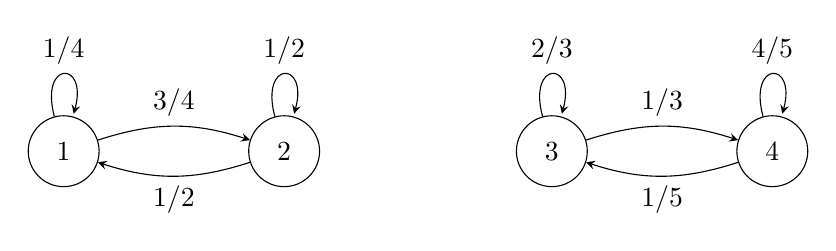
\begin{tikzpicture}[>=stealth]
\node[circle, draw, minimum size=0.9cm] (1) at (0,0) {1};
\node[circle, draw, minimum size=0.9cm] (2) at (2.8,0) {2};
\node[circle, draw, minimum size=0.9cm] (3) at (6.2,0) {3};
\node[circle, draw, minimum size=0.9cm] (4) at (9,0) {4};

\draw[->] (1) edge[loop above] node {$1/4$} (1);
\draw[->] (1) edge[bend left=18] node[above] {$3/4$} (2);
\draw[->] (2) edge[bend left=18] node[below] {$1/2$} (1);
\draw[->] (2) edge[loop above] node {$1/2$} (2);

\draw[->] (3) edge[loop above] node {$2/3$} (3);
\draw[->] (3) edge[bend left=18] node[above] {$1/3$} (4);
\draw[->] (4) edge[bend left=18] node[below] {$1/5$} (3);
\draw[->] (4) edge[loop above] node {$4/5$} (4);
\end{tikzpicture}
\end{center}

\begin{subprob}(4 pts)
Find the adjacency matrix $A$ for this Markov chain. \\

$A = $ \minibox{8cm}{$\begin{bmatrix}
    1/4 & 1/2 & 0 & 0\\
    3/4 & 1/2 & 0 & 0\\
    0 & 0 & 2/3 & 1/5\\
    0 & 0 & 1/3 & 4/5
    \end{bmatrix}$}[6cm]

\begin{solution}
Column $j$ contains the probabilities of transitioning from state $j$ to all other states; columns must sum to $1$. Reading from the diagram, the first two columns come from the left ``connected component" (made up of states $1$ and $2$), and the last two columns come from the right connected component. So
\[
\boxed{
A =
\begin{bmatrix}
1/4 & 1/2 & 0 & 0\\
3/4 & 1/2 & 0 & 0\\
0 & 0 & 2/3 & 1/5\\
0 & 0 & 1/3 & 4/5
\end{bmatrix}}
\]
\end{solution}
\end{subprob}

\begin{subprob}(6 pts) Suppose the chain starts in \textbf{state $\mathbf{1}$}. Fill each box with the \textbf{long-run fraction} of time spent in each state. Your answers should be numbers with no variables, and should sum to $1$. \\

State 1: \minibox{2cm}{$2/5$}[1.5cm] \quad State 2: \minibox{2cm}{$3/5$}[1.5cm] \quad State 3: \minibox{2cm}{$0$}[1.5cm] \quad State 4: \minibox{2cm}{$0$}[1.5cm]

\begin{solution}
As we know from \href{https://notes.eecs245.org/eigenvalues-and-eigenvectors/markov-chains-adjacency-matrices/}{Chapter 9.3}, the long-run fraction of time spent in each state is described by the eigenvector of the adjacency matrix corresponding to eigenvalue $1$ (and whose components sum to $1$). \\

What is tricky about this particular adjacency matrix is that it has \textbf{two linearly independent eigenvectors, both for the eigenvalue $1$.} Why? Note that the Markov chain has two isolated islands, and its impossible to transition between them. So if we ever start in states $1$ or $2$, in the long run, we will only spend time in states $1$ and $2$. Similarly, if we start in states $3$ or $4$, in the long run, we will only spend time in states $3$ and $4$. \\

This means that we can simplify the problem by just looking at the $2 \times 2$ matrix in the top right of $A$ corresponding to the left island (states $1$ and $2$). This matrix is

$$A_{\text{left}} = \begin{bmatrix} 
1/4 & 1/2 \\
3/4 & 1/2
\end{bmatrix}
$$

All we need to do now is find the eigenvector of $A_{\text{left}}$ corresponding to eigenvalue $1$. If such an eigenvector is of the form $\begin{bmatrix} a \\ b \end{bmatrix}$, then
\[
\begin{bmatrix} 1/4 & 1/2 \\ 3/4 & 1/2 \end{bmatrix} \begin{bmatrix} a \\ b \end{bmatrix} = 1 \begin{bmatrix} a \\ b \end{bmatrix}
\]

The first row gives us

$$\frac{1}{4}a + \frac{1}{2} b = a \implies \frac{1}{2} b = \frac{3}{4}a \implies b = \frac{3}{2}a$$

So, if $a = 2$, then $b = 3$. But, the steady-state distribution must have components that sum to $1$, so as probabilities, we're looking at $2/5$ and $3/5$. \\

Not only is $\begin{bmatrix} 2/5 \\ 3/5 \end{bmatrix}$ an eigenvector of $A_{\text{left}}$ corresponding to eigenvalue $1$, but

$$\begin{bmatrix} 2/5 \\ 3/5 \\ 0 \\ 0 \end{bmatrix}$$

is an eigenvector of the full matrix $A$ corresponding to eigenvalue $1$! The 0's in the latter two components effectively ``ignore'' states $3$ and $4$, representing the assumption that we start in state $1$. \\

So, if we start in state $1$,
\[
\boxed{\text{State 1: } \frac{2}{5},\quad \text{State 2: } \frac{3}{5},\quad \text{State 3: } 0,\quad \text{State 4: } 0}
\]

In case you're curious, the other linearly independent eigenvector of $A$ corresponding to eigenvalue $1$ is

$$\begin{bmatrix} 0 \\ 0 \\ 3/8 \\ 5/8 \end{bmatrix}$$

There's a section in \href{https://notes.eecs245.org/eigenvalues-and-eigenvectors/multiplicities-diagonalization/\#example-another-diagonalizable-matrix}{Chapter 9.4} about block diagonal matrices that is relevant here.

\end{solution}
\end{subprob}

% \begin{subprob}
% As $k \to \infty$, what does $A^k$ converge to?

% Find $\lim_{k \to \infty} A^k$.
% \end{subprob}

\newpage

Now, consider a \textbf{modified} version of the Markov chain. Changes have been emphasized in \textbf{bold}.

\begin{center}
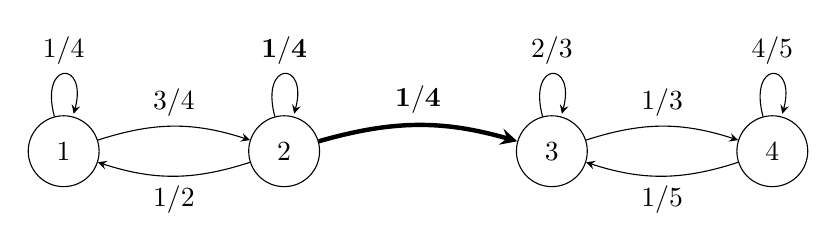
\begin{tikzpicture}[>=stealth]
\node[circle, draw, minimum size=0.9cm] (1) at (0,0) {1};
\node[circle, draw, minimum size=0.9cm] (2) at (2.8,0) {2};
\node[circle, draw, minimum size=0.9cm] (3) at (6.2,0) {3};
\node[circle, draw, minimum size=0.9cm] (4) at (9,0) {4};

\draw[->] (1) edge[loop above] node {$1/4$} (1);
\draw[->] (1) edge[bend left=18] node[above] {$3/4$} (2);
\draw[->] (2) edge[bend left=18] node[below] {$1/2$} (1);
\draw[->] (2) edge[loop above] node {$\mathbf{1/4}$} (2);
\draw[->, ultra thick] (2) edge[bend left=16] node[above] {$\mathbf{1/4}$} (3);

\draw[->] (3) edge[loop above] node {$2/3$} (3);
\draw[->] (3) edge[bend left=18] node[above] {$1/3$} (4);
\draw[->] (4) edge[bend left=18] node[below] {$1/5$} (3);
\draw[->] (4) edge[loop above] node {$4/5$} (4);
\end{tikzpicture}
\end{center}

\begin{subprob}(4 pts)
Consider the statement: ```If we start in \_\_\_\_, the long-run fraction of time spent in each state is the same as in the original chain.'' \\

Which of the following could be placed in the blank to make the statement true? \textbf{Select all} that apply. \\

\squarebubble{state 1} \squarebubble{state 2} \correctsquarebubble{state 3} \correctsquarebubble{state 4} \squarebubble{none of these are valid}

% Fill each box with the \textbf{long-run fraction} of time spent in each state. Your answers should be numbers with no variables, and should sum to $1$. \textit{Hint: Work efficiently!} \\

% State 1: \minibox{2cm}{}[1.5cm] \quad State 2: \minibox{2cm}{}[1.5cm] \quad State 3: \minibox{2cm}{}[1.5cm] \quad State 4: \minibox{2cm}{}[1.5cm]

\begin{solution}
In the modified chain, starting in state $1$ or state $2$ eventually leads to the right connected component, because there is now a positive-probability path from state $2$ to state $3$. This changes the long-run fractions compared to the original chain. The long-run fraction of time spent in states $1$ and $2$ now will be $0$. \\

Starting in state $3$ or state $4$, the chain stays in the right connected component, and that component has not changed. There is no way to go from state $3$ to $2$ or $1$. So, the long-run fractions are the same as in the original chain; $3/8$ for state $3$ and $5/8$ for state $4$, and $0$ for states $1$ and $2$. \\

The correct choices are
\[
\boxed{\text{state 3 and state 4}}
\]
\end{solution}
\end{subprob}

\end{prob}

\begin{prob}[(10 pts)]
Let $S$ be a $3 \times 3$ \textbf{symmetric} matrix with eigenvectors $\vec v_1$, $\vec v_2$, and $\vec v_3$ corresponding to eigenvalues $5$, $2$, and $-1$, respectively. Assume that each $\vec v_i$ is a unit vector.

Suppose $\vec x \in \mathbb{R}^3$ and that
\[
\vec x = 3\vec v_1 - 4\vec v_2 + \vec v_3
\]

\begin{subprob}(6 pts)
Write $S^2 \vec x$ as a linear combination of $\vec v_1$, $\vec v_2$, and $\vec v_3$. Fill in each box with a number with no variables. \\

\noindent $S^2 \vec x = \minibox{2cm}{$75$}[1cm] \: \vec v_1 + \minibox{2cm}{$-16$}[1cm] \: \vec v_2 + \minibox{2cm}{$1$}[1cm] \: \vec v_3$

\begin{solution}
Applying $S^2$ multiplies each eigenvector by the square of its eigenvalue, so
\[
S^2\vec x
=
3(5^2)\vec v_1 - 4(2^2)\vec v_2 + ((-1)^2)\vec v_3
=
\boxed{75\vec v_1 - 16\vec v_2 + \vec v_3}
\]
This result doesn't rely on the fact that $\vec v_1$, $\vec v_2$, and $\vec v_3$ are unit vectors or orthogonal; we'll use these assumptions in the next part.
\end{solution}
\end{subprob}

\begin{subprob}(4 pts)
What is the value of $\lVert S\vec x \rVert^2$?

\bubble{$24$} \bubble{$26$} \bubble{$218$} \correctbubble{$290$} \bubble{$5882$} \bubble{Not enough information}

\begin{solution}
Applying $S$ once gives
\[
S\vec x = 15\vec v_1 - 8\vec v_2 - \vec v_3
\]
Since $S$ is symmetric, eigenvectors corresponding to distinct eigenvalues are orthogonal. The vectors $\vec v_1$, $\vec v_2$, and $\vec v_3$ are also unit vectors, so

\begin{align*}
\lVert S\vec x \rVert^2 &= \lVert 15\vec v_1 - 8\vec v_2 - \vec v_3 \rVert^2 \\
&= (15 \vec v_1 - 8\vec v_2 - \vec v_3) \cdot (15\vec v_1 - 8\vec v_2 - \vec v_3) \\
&= 15^2 \underbrace{(\vec v_1 \cdot \vec v_1)}_{1} - 8 \cdot 15 \underbrace{(\vec v_1 \cdot \vec v_2)}_{0} - 15 (\vec v_1 \cdot \vec v_3) \\
& \quad - 8 \cdot 15 (\vec v_2 \cdot \vec v_1) + 8^2 (\vec v_2 \cdot \vec v_2) + 8 (\vec v_2 \cdot \vec v_3) \\
& \quad - (\vec v_3 \cdot \vec v_1) - 8 (\vec v_3 \cdot \vec v_2) + (-1)^2(\vec v_3 \cdot \vec v_3) \\
&= 15^2 + 8^2 + 1^2 \\
&= 290
\end{align*}

Yet another way to look at this is to see that $S = Q \Lambda Q^T$, where the columns of $Q$ are the vectors $\vec v_i$ and the diagonal entries of $\Lambda$ are $5$, $2$, and $-1$. So,

\begin{align*}
\lVert S\vec x \rVert^2 
  &= \vec x^T S^T S \vec x \\
  &= \vec x^T S^2 \vec x \\
  &= \vec x^T (Q \Lambda Q^T)^2 \vec x \\
  &= \vec x^T Q \Lambda^2 Q^T \vec x \\
  &= \vec x^T Q 
    \begin{bmatrix}
      25 & 0 & 0 \\
      0 & 4 & 0 \\
      0 & 0 & 1
    \end{bmatrix}
    Q^T \vec x \\
  &= \begin{bmatrix} 3 & -4 & 1 \end{bmatrix}
  \begin{bmatrix}
    25 & 0 & 0 \\
    0 & 4 & 0 \\
    0 & 0 & 1
  \end{bmatrix}
  \begin{bmatrix} 3 \\ -4 \\ 1 \end{bmatrix} \\
  &= \boxed{290} 
\end{align*}

In this solution, we used the fact that $\vec x = 3 \vec v_1 - 4 \vec v_2 + \vec v_3 = Q \begin{bmatrix} 3 \\ -4 \\ 1 \end{bmatrix}$, and since $Q^T Q = I$ (if $Q$'s columns are the orthonormal $\vec v_i$'s), then $Q^T \vec x = Q^TQ \begin{bmatrix} 3 \\ -4 \\ 1 \end{bmatrix} = \begin{bmatrix} 3 \\ -4 \\ 1 \end{bmatrix}$.

\end{solution}

\end{subprob}

\end{prob}

\newpage

\begin{prob}[(12 pts)]
Suppose $\tilde X$ is an $n \times 2$ matrix whose columns are mean-centered (i.e. have a mean of 0). Furthermore, suppose 
$$\tilde X^T \tilde X = \begin{bmatrix} 3 & 2 \\ 2 & 6 \end{bmatrix}$$
Note that $\tilde X^T \tilde X$ has eigenvalues of $7$ and $2$. Let $\tilde X = U \Sigma V^T$ be the singular value decomposition of $\tilde X$, and let $\vec v_1$ be the first column of $V$ (not $V^T$).

\begin{subprob}(4 pts) What is $\vec v_1$? Give your answer as a vector with no variables. If there are multiple correct answers, you only need to provide one. \\

$\vec v_1 = \minibox{3cm}{$\frac{1}{\sqrt 5}\begin{bmatrix}1\\2\end{bmatrix}$}[4cm]$
\begin{solution}
The first right singular vector, $\vec v_1$, is an eigenvector of $\tilde X^T\tilde X$ corresponding to the largest eigenvalue, $7$. So we solve
\[
\begin{bmatrix}
3 & 2\\
2 & 6
\end{bmatrix}
\begin{bmatrix}
a\\b
\end{bmatrix}
=
7
\begin{bmatrix}
a\\b
\end{bmatrix}
\]
The first row gives
\[
3a+2b=7a
\implies
b=2a
\]
One unit vector in this direction is
\[
\vec v_1 = \boxed{\frac{1}{\sqrt 5}\begin{bmatrix}1\\2\end{bmatrix}}
\]
\end{solution}
\end{subprob}

\begin{subprob}(3 pts) Suppose the variance of the \textbf{second} principal component is $1/15$. What is $n$, the number of rows in $\tilde X$? Give your answer as a number with no variables. \\

$n = \minibox{3cm}{$30$}[1cm]$

\begin{solution}
The variance of the second principal component is
\[
\frac{\sigma_2^2}{n}
\]
Since $\sigma_2^2$ is the second-largest eigenvalue of $\tilde X^T\tilde X$, we have $\sigma_2^2=2$. So
\[
\frac{2}{n}=\frac{1}{15}
\]
This gives
\[
n=\boxed{30}
\]
\end{solution}
\end{subprob}

\begin{subprob}(5 pts)
Suppose that $\vec u_2$ is the second column of $U$, corresponding to the singular value $\sigma_2$, in the singular value decomposition of $\tilde X$.

Prove that $\tilde X \vec v_1$ and $\sigma_2 \vec u_2$ are orthogonal. You do not need to re-prove any facts about the singular value decomposition, but you should state any facts you use. \\

\emptybox{7cm}

\begin{solution}
Using the SVD relationship,
\[
\tilde X\vec v_1 = \sigma_1\vec u_1
\]
So
\[
(\tilde X\vec v_1)^T(\sigma_2\vec u_2)
=
(\sigma_1\vec u_1)^T(\sigma_2\vec u_2)
=
\sigma_1\sigma_2 \vec u_1^T\vec u_2
\]
The columns of $U$ are orthonormal, so $\vec u_1^T\vec u_2=0$. Therefore,
\[
(\tilde X\vec v_1)^T(\sigma_2\vec u_2)=0
\]
This proves that $\tilde X\vec v_1$ and $\sigma_2\vec u_2$ are orthogonal.
\end{solution}

\end{subprob}

\end{prob}

% \begin{prob}[(XX pts)]
% Let $\tilde X$ be a centered $5 \times 2$ data matrix. Consider the two unit directions
% \[
% \vec v_1 =
% \frac{1}{\sqrt 5}
% \begin{bmatrix}
% 2\\
% 1
% \end{bmatrix},
% \qquad
% \vec v_2 =
% \frac{1}{\sqrt 5}
% \begin{bmatrix}
% 1\\
% -2
% \end{bmatrix}
% \]

% Suppose
% \[
% \tilde X \vec v_1 =
% \begin{bmatrix}
% 4\\
% 2\\
% 0\\
% -2\\
% -4
% \end{bmatrix},
% \qquad
% \tilde X \vec v_2 =
% \begin{bmatrix}
% 0\\
% 1\\
% -2\\
% 1\\
% 0
% \end{bmatrix}
% \]

% \begin{subprob}(XX pts)
% Which direction, $\vec v_1$ or $\vec v_2$, captures more variance? How much squared variance does that direction capture? \\

% \noindent Direction: \minibox{3cm}{$\vec v_1$}[0.8cm] \qquad Squared variance captured: \minibox{3cm}{$40$}[0.8cm]

% \end{subprob}

% \begin{subprob}(XX pts)
% Suppose $\vec v_1$ is the first right singular vector of $\tilde X$. Find the first singular value $\sigma_1$ and the corresponding left singular vector $\vec u_1$. \\

% \[
% \sigma_1 = \minibox{3cm}{$2\sqrt{10}$}[0.8cm]
% \qquad
% \vec u_1 =
% \minibox{4cm}{$\frac{1}{\sqrt{10}}\begin{bmatrix} 2 \\ 1 \\ 0 \\ -1 \\ -2 \end{bmatrix}$}[2cm]
% \]

% \end{subprob}

% \begin{subprob}(XX pts)
% What proportion of the total variance is explained by the first principal component? Give your answer as a simplified fraction.

% \[
% \minibox{4cm}{$\frac{20}{23}$}[0.8cm]
% \]

% \end{subprob}

% \end{prob}

\newpage

\begin{prob}[(4 pts)]
What is one topic you studied a lot for that wasn't on the Final Exam? \textbf{Blank answers will receive no credit!}

\emptybox{4cm}
\begin{solution}
One topic that didn't appear was convexity --- there was originally going to be a question about convexity but we cut it to prevent the exam from being too long.
\end{solution}
\end{prob}

Congrats on completing the Final Exam for EECS 245! We'll really miss you; please stay in touch.

Feel free to draw us a picture about EECS 245 in the box below. 

\emptybox{8cm}

\vfill

Did you notice any violations of the Honor Code during the exam? If so, share details with us here. We will keep your identity anonymous when investigating any cases.

\emptybox{3cm}
\end{document}
